\documentclass[12pt,a4paper,fleqn]{article}
\usepackage{rmpackages}																% usual packages
\usepackage{rmtemplate}																% graphic charter
\usepackage{rmexocptce}																% for DS with cptce eval

%\cfoot{} 													% if no page number is needed
%\renewcommand\arraystretch{1.5}		% stretch table line height

\begin{document}

\normalem

\begin{header}
Chapitre 11 -- Transformations chimiques
\end{header}

\section{Quelques transformations}

\subsection{Combustion du carbone}

Pour revoir l'expérience : \href{https://youtu.be/zu7revUCefw?t=398}{https://youtu.be/zu7revUCefw?t=398}.

\begin{multicols}{2}

\begin{center}
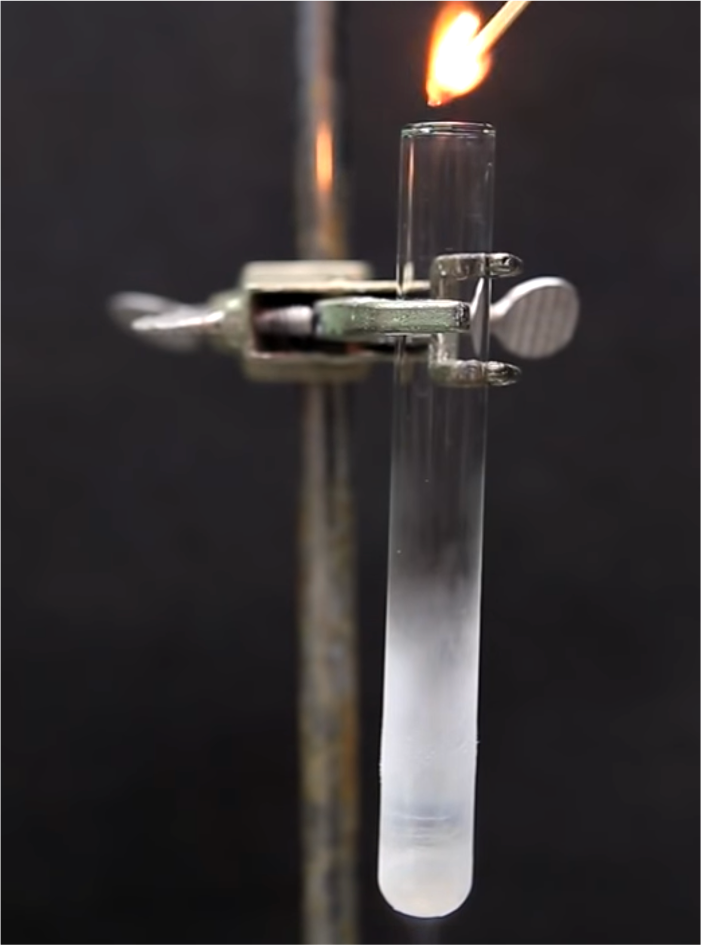
\includegraphics[width=\linewidth/2]{images/c_in_o2.png}
\end{center}

\emph{Quel est ce liquide ?}

\begin{center}
\begin{tikzpicture}
\draw [color=white] (0,0.25) -- ++ (.99\linewidth, 0);
\draw [color=gray_c] (0,0) -- ++ (.99\linewidth, 0);
\end{tikzpicture}
\end{center}

\vfill

\begin{center}
\begin{tikzpicture}
\draw [color=green_f] (0,0) -- ++ (.4\linewidth, 0) node [midway, below] {État initial} --++ (0,3) --++ (-.4\linewidth,0) --++ (0,-3);
\draw [color=green_f] (.59\linewidth,0) -- ++ (.4\linewidth, 0) node [midway, below] {État final} --++ (0,3) --++ (-.4\linewidth,0) --++ (0,-3);
\draw [->,>=stealth, thick] (.45\linewidth,1.5) --++ (.1\linewidth,0);
\end{tikzpicture}
\end{center}
\end{multicols}

\paragraph{Équation de réaction :}

\begin{center}
\begin{tikzpicture}
\draw [color=white] (0,1) -- ++ (.99\linewidth, 0);
\draw [color=gray_c] (0,0) -- ++ (.99\linewidth, 0);
\draw [color=white] (0,-2) -- ++ (.99\linewidth, 0);
\end{tikzpicture}
\end{center}
Une espèce qui n'intervient pas dans l'équation de réaction s'appelle une espèce \phantom{spectatrice spectatrice}.

\subsection{Combustion du méthane}

\emph{En plus du dioxyde de carbone, quelle espèce se forme lors de la combustion du méthane ?}

\begin{center}
\begin{tikzpicture}
\draw [color=white] (0,0.25) -- ++ (.99\linewidth, 0);
\draw [color=gray_c] (0,0) -- ++ (.99\linewidth, 0);
\end{tikzpicture}
\end{center}

\paragraph{Équation de réaction :}

\begin{center}
\begin{tikzpicture}
\draw [color=white] (0,1) -- ++ (.99\linewidth, 0);
\draw [color=gray_c] (0,0) -- ++ (.99\linewidth, 0);
\end{tikzpicture}
\end{center}

\newpage
\subsection{Équilibrer une équation de réaction}

\emph{Vérifier que l'équation de réaction ci-dessous est équilibrée.}

\begin{center}
$\mathrm{2~C_2H_6 \quad + \quad 7~O_2 \quad \rightarrow \quad 4~CO_2 \quad + \quad 6~H_2O} $
\end{center}

\vspace{2cm}

\emph{Équilibrer les équations de réactions ci-dessous.}
\begin{multicols}{2}
\begin{enumerate}
\begin{spacing}{1.5}
\item[•] $\mathrm{...~H_2O + ...~Cl_2 \rightarrow ...~HCl + ...~HClO}$

\item[•] $\mathrm{...~Mg + ...~SiO_2\rightarrow ...~MgO + ...~Si} $

\item[•] $\mathrm{...~Pb^{2+} + ...~I^- \rightarrow ...~PbI_2}$

\item[•] $\mathrm{...~Fe + ...~ Cl_2 \rightarrow ...~Fe^{3+} + ...~Cl^-}$
\end{spacing}
\end{enumerate}
\end{multicols}

Lors d'une réaction chimique, il y a conservation :
\begin{spacing}{1.5}
\begin{itemize}
\item[•]

\item[•]
\end{itemize}
\end{spacing}

\subsection*{Applications}

\subsubsection*{Le dihydrogène}

Le dihydrogène ($\mathrm{H_2}$) peut réagir avec le dioxygène pour former de l'eau.
Écrire l'équation de cette réaction.
Une réaction détonante : \href{https://youtu.be/ce6imsXTkGQ?t=16}{https://youtu.be/ce6imsXTkGQ?t=16}.
\begin{center}
\begin{tikzpicture}
\draw [color=white] (0,1) -- ++ (.99\linewidth, 0);
\draw [color=gray_c] (0,0) -- ++ (.99\linewidth, 0);
\end{tikzpicture}
\end{center}

\subsubsection*{Attaque d'un métal par un acide}

\begin{multicols}{2}
\begin{center}
\begin{tikzpicture}
\draw [color=green_f] (0,0) -- ++ (.45\linewidth, 0) node [midway, below] {État initial} --++ (0,2.5) --++ (-.45\linewidth,0) --++ (0,-2.5);
\draw (.01\linewidth, 2) node [right] {Zinc : $\mathrm{Zn}$};
\draw (.01\linewidth, 1.5) node [right] {Ion hydrogène : $\mathrm{H^+}$};
\draw (.01\linewidth, 1) node [right] {Ion chlorure : $\mathrm{Cl^-}$};
\draw (.01\linewidth, .5) node [right] {Eau : $\mathrm{H_2O}$};

\draw [color=green_f] (.59\linewidth,0) -- ++ (.4\linewidth, 0) node [midway, below] {État final} --++ (0,2.5) --++ (-.4\linewidth,0) --++ (0,-2.5);
\draw (.6\linewidth, 2) node [right] {Ion zinc : $\mathrm{Zn^{2+}}$};
\draw (.6\linewidth, 1.5) node [right] {Dihydrogène : $\mathrm{H_2}$};
\draw (.6\linewidth, 1) node [right] {Ion chlorure : $\mathrm{Cl^-}$};
\draw (.6\linewidth, .5) node [right] {Eau : $\mathrm{H_2O}$};

\draw [->,>=stealth, thick] (.475\linewidth,1.25) --++ (.1\linewidth,0);
\end{tikzpicture}
\end{center}

Identifier :
\begin{itemize}
\item[•] les produits :
\item[•] les réactifs :
\item[•] les espèces spectatrices :
\end{itemize}
\end{multicols}

Écrire l'équation de cette réaction.
\begin{center}
\begin{tikzpicture}
\draw [color=white] (0,1) -- ++ (.99\linewidth, 0);
\draw [color=gray_c] (0,0) -- ++ (.99\linewidth, 0);
\end{tikzpicture}
\end{center}

\section{Bilan de quantité de matière}

On reprend l'exemple de la combustion du carbone $ \mathrm{C + {\color{red}O_2} \rightarrow {\color{gray}CO_2}}$. 
Cette équation de réaction indique qu'\textbf{un} atome de carbone réagit avec \textbf{une} molécule de dioxygène pour former \textbf{une} molécule de dioxyde de carbone.
S'il y a moins d'atomes de carbone que de molécules de dioxygène, la réaction s'arrête quand tout le carbone a été consommé.

\begin{center}
\newcommand{\carbon}[1]{\fill #1 rectangle ++(1,1);}
\newcommand{\dioxygen}[1]{\fill [color=red] #1 rectangle ++(1,1);}
\newcommand{\gaz}[1]{\fill [color=gray] #1 rectangle ++(1,1);}

\begin{tikzpicture}
\draw [color=green_f] (0,0) -- ++ (.4\linewidth, 0) node [midway, below] {État initial} --++ (0,3) --++ (-.4\linewidth,0) --++ (0,-3);
\draw [color=green_f] (.59\linewidth,0) -- ++ (.4\linewidth, 0) node [midway, below] {État final} --++ (0,3) --++ (-.4\linewidth,0) --++ (0,-3);
\draw [->,>=stealth, thick] (.45\linewidth,1.5) --++ (.1\linewidth,0);

\carbon{(1,1)};
\dioxygen{(3.5,1.75)};
\dioxygen{(5,1.75)};
\dioxygen{(3.5,.25)};
\dioxygen{(5,.25)};

\gaz{(11,1)};
\dioxygen{(15,1.75)};
\dioxygen{(13.5,1)};
\dioxygen{(15,.25)};
\end{tikzpicture}
\end{center}

Lors d'une transformation chimique totale, l'un au moins des réactifs est entièrement consommé : c'est le \textbf{réactif limitant}.
Dans l'exemple ci-dessus, le réactif limitant est le \textcolor{gray_c}{\underline{\phantom{carbone carbone}}}.

Si les deux réactifs sont entièrement consommés, ils ont été mélangés dans les \textbf{proportions stœchiométriques} : on dit que le mélange est \textbf{stœchiométrique}.

\subsection*{Application}

\emph{Rappeler l'équation de la réaction de combustion du méthane.}
\begin{center}
\begin{tikzpicture}
\draw [color=white] (0,0.25) -- ++ (.99\linewidth, 0);
\draw [color=gray_c] (0,0) -- ++ (.99\linewidth, 0);
\end{tikzpicture}
\end{center}

\emph{En utilisant le même mode de représentation que l'exemple précédent, schématiser cette transformation dans le cas où les réactifs ont été introduits dans les proportions stœchiométriques.}

\begin{center}
\begin{tikzpicture}
\draw [color=green_f] (0,0) -- ++ (.4\linewidth, 0) node [midway, below] {État initial} --++ (0,3) --++ (-.4\linewidth,0) --++ (0,-3);
\draw [color=green_f] (.59\linewidth,0) -- ++ (.4\linewidth, 0) node [midway, below] {État final} --++ (0,3) --++ (-.4\linewidth,0) --++ (0,-3);
\draw [->,>=stealth, thick] (.45\linewidth,1.5) --++ (.1\linewidth,0);
\end{tikzpicture}
\end{center}

\section{Caractère exothermique ou endothermique d'une transformation}

La plupart des transformations chimiques s'accompagnent d'un transfert d'énergie :
\begin{itemize}
\item[•] on dit qu'une transformation est \textbf{exothermique} si elle \textbf{libère} de l'énergie : la transformation s'accompagne d'une \textbf{augmentation} de température (ex : combustion, dissolution de la soude);
\item[•] à l'inverse, on dit qu'une transformation est \textbf{endothermique} si elle \textbf{reçoit} de l'énergie : la transformation s'accompagne d'une \textbf{diminution} de température (ex : dissolution du nitrate d'ammonium).
\end{itemize}

\section{Synthèse d'une espèce chimique}

Cf. TP -- Comme un parfum de lavande.



\end{document}